\documentclass[a4paper, fleqn]{article}
\usepackage{chemfig}
\usepackage{mhchem}
\usepackage{xcolor}
\usepackage{amsmath}
\usepackage{tikz}
\usepackage{chemfig}
\usepackage{amssymb}
\usepackage{hyperref}
\usepackage[
  left=1cm,
  right=1cm,
  top=2cm,
  bottom=2cm,
]{geometry}

\begin{document}
\tableofcontents
\newpage
\section{Thermodynamik für Knechte}
\subsection{Was ist Thermodynamik?}
Thermodynamik:
\begin{itemize}
    \item makroskopische Skala
    \item Umwandlungen von Energie
    \begin{itemize}
        \item Austausch von Wärme
        \item Leistung von Arbeit
    \end{itemize}
    \item Gleichgewicht
    \item Richtung von spontanen Prozessen
\end{itemize}
Chemische Thermodynamik: Lage der chemischen Gleichgewichte\\
\hspace*{1cm} Wärmeeffekte dhemischer Reaktionen\\
Technische Thermodynamik: Umsetzung von Wärme und Arbeit\\
\begin{equation*}
    \ce{N2 + 3H2 -> 2NH3}    
\end{equation*}
\begin{center}
    250$-$300 bar\\
    450$-$550°
\end{center}
\ce{MeOH} Automobilantrieb:\\
\ce{CH3OH + \frac{3}{2}O2 -> CO2 + H2O}\\
\\
Anode\\
\hspace*{1cm} \ce{CH3OH + H2O -> 6H+ + 6e- + CO2}\\
Kathode\\
\hspace*{1cm} \ce{\frac{3}{2}O2 + 6H+ + 6e- -> 3H2O}\\
\subsection{Thermodynamische Systeme}
Definitionen:\\
\underline{System:} \hspace*{1.55cm} Der Teil des Universums, der uns interessiert\\
\underline{Umgebung:} \hspace*{1cm} Der Rest \hspace*{0.5cm} (der im Kontakt mit dem System steht)\\
\\
Grenze ist die \underline{Systemgrenze} \hspace*{0.5cm} (Wand)
\begin{center}
    \begin{tabular}{c c c} 
     \hline
     System & Materienaustausch & Energieaustausch \\ 
     \hline
     isoliert & $-$ & $-$ \\ 
     geschlossem & $-$ & $+$ \\ 
     offen & $+$ & $+$\\
     \hline
    \end{tabular}
    \end{center}
\subsubsection{Phase}
Bereich ohne Sprunghafte Änderung
\begin{itemize}
    \item chemische Zusammensetzung
    \item physikalische Eigenschaften
    \item Aggregatzustände
\end{itemize}
Komponenten
\begin{itemize}
    \item chemisch unterscheidbare Bestandteile (Stoffe)
\end{itemize}
Modifikationen von Elementen: Allotrope
\subsubsection{Aggregatzustände}
\begin{itemize}
    \item Teilchenabstand
    \item Teilchenordnung
\end{itemize}
$R$ ist der Abstand zwischen den Zentren zweier Atome, und $d$ ist der Durchmessser eines Atomes.\\
Gasförmig:\\
$R >> d$\\
keine Ordnung\\
\\
Flüssig:\\
$R \approx d$\\
Nahordnung\\
\\
Fest:\\
$R \approx d$\\
Fernordnung = Kristallin\\
Nahordnung = Amorph\\
\\
Es gibt noch Plasma, dabei haben sich Elektronen und Atomkerne separiert\\
\subsubsection{Gleichgewicht}
Mechanisch:
\begin{equation*}
    \sum \vec{F} = 0, \sum \vec{\tau} = 0
\end{equation*}
Anmerkung $\tau$ ist hier das Drehmoment\\\\
Thermisch:
\begin{equation*}
    \Delta T = T_{ex} - T_{in} = 0
\end{equation*}
\\
Chemisch:\\
Chemische Potentiale \textcolor{gray}{(von Edukten/Produkten)} sind gleich.\\
\begin{center}
    Dynmaisches Gleichgewicht $\leftrightarrow$ Fließgleichgewicht
\end{center}
\subsubsection{0. Hauptsatz der Thermodynamik}
\begin{equation*}
    T_a \neq T_b \neq T_c -\Delta E -> T_a = T_b = T_c
\end{equation*}
$T_a = T_b$\\
a,b im thermischen Gleichgewicht\\\\
und $T_b = T_c$\\
b,c im thermischen GLeichgewicht\\\\
dann muss auch $T_a = T_b$ gelten\\
a,c im thermischen Gleichgewicht.\\\\
TD: thermodynamische oder absolute Temperatur $T$[K]\\
Celsiustemperatur $\vartheta$[°C]\\
$\vartheta$ = $T$ - 273,15
\subsection{Zustandsgrößen}
\underline{Zustand:}\\
\hspace*{1cm}Beschaffenheit des Systems\\
\hspace*{1.5cm}$\rightarrow$Alle Infos um das System eindeutig beschreiben zu können\\\\
\underline{Zustandsgrößen:}\\
\hspace*{1cm} $T, V, p, H$ \textcolor{gray}{(Enthalpie)} $, S$ \textcolor{gray}{(Entropie)}\\
\hspace*{1cm} Änderungen sind wegunabhängig: $\left|\Delta A \right|$\\\\
\underline{Prozessgrößen:}\\
\hspace*{1cm} $q$ \textcolor{gray}{(Wärme)}, $W$ \textcolor{gray}{(Arbeit)}, $F$ \textcolor{gray}{(Kraft)} beschreiben Zustandsänderungen\\
\subsubsection{intensive Zustandsgrößen \textcolor{gray}{(unabhängig von der Stoffmenge $n$ - \underline{in}dependent)}}
Temperatur $T$\\
Druck $p$\\
Dichte $\rho$\\
Viskosität $\eta$\\
\subsubsection{extensive Zustandsgrößen \textcolor{gray}{(abhängig von der Stoffmenge $n$)}}
Volumen $V$\\
Stoffmenge $n$\\
Innere Energie $U$\\
Entropie $S$\\
\subsubsection{Definition einer spezifische Größe \textcolor{gray}{(teilen durch Masse)}}
spezifisches Volumen $v$ = $\frac{V}{m}$
\subsubsection{Definition einer molaren Größe \textcolor{gray}{(teilen durch Stoffmenge)}}
molares Volumen $V_m$ = $\frac{V}{n}$
\subsubsection{verschiedene Größen}
Molmasse $M$ [$\frac{\mathrm{g}}{\mathrm{mol}}$]\\
1 Mol Tielchen = $6, 02 \cdot 10^{23}$ Teilchen\\
$N_A = 6.02 \cdot 10^{23} \frac{1}{\mathrm{mol}}$\\\\
Stoffmenge $n$ [mol] $=\frac{N}{N_\eta}=\frac{\mathrm{Masse}}{\mathrm{Molmasse}}=\frac{m}{M}$\\\\
Konzentration $c$ [$\frac{\mathrm{mol}}{\mathrm{l}}$] $= \frac{n}{V}$\\\\
Dichte $\rho$ [$\frac{\mathrm{kg}}{\mathrm{m}^3}$]\\\\
Molalität $b$ [$\frac{\mathrm{mol}}{\mathrm{kg}}$] $=\frac{\mathrm{Stoffmenge}}{\mathrm{Masse_{L\text{ö}M}}}=\frac{n}{m_{LM}}$\\\\
Partielle Größen\\
Molenbruch\\
\begin{equation*}
    x_i=\frac{n_i}{\sum_i n_i}
\end{equation*}
\subsubsection{thermodynamische Prozesse}
\begin{itemize}
    \item Volumenänderung ("Arbeit") $w = -p \Delta V$
    \item Temperatruänderung ("Wärmeaustausch") $q = c \delta T$ hierbei: $c =$ Wärmekapazität
    \item Phasenübergänge $q = \Delta H$
    \item chemische Reaktionen \ce{2A + B -> c}\\ \begin{equation*}
        n_c(t)=n_c(0)+\nu_i\xi
    \end{equation*}\\hierbei $\nu =$ Stöchiometrischer Koeffizient und $\xi =$ Reaktionsfortschritt
\end{itemize}
\begin{center}
    Prozessführung
    \begin{tabular}{c c c} 
        \hline
        Bezeichnung & Konstante Größe & Fachbegriff und Beschreinbung \\ 
        \hline
        Isotherm & $T$ & adiabatisch: ohne Wärmeaustausch \\ 
        Isobar & $p$ & reversibel: im ständigen Gleichgewicht\\ 
        Isochor & $V$ & irreversibel: nicht im Gleichgewicht\\
        \hline
       \end{tabular}
\end{center}
\subsection{Zustandsgleichung - Zusammenhang zwischen Zustandsgrößen}
\begin{equation*}
    A = B^2 + 3C
\end{equation*}
A ist hierbei die Zustandsgröße, B und C sin Zustandsvariablen.\\
Beispiel:
\begin{equation*}
    p = \frac{nRT}{V}
\end{equation*}
\\
\textbf{Totales Differential:}\\
\begin{equation*}
    Z = f(x,y)
\end{equation*}
\begin{equation*}
    dz=\left(\frac{\partial z}{\partial x}\right)_ydx+\left(\frac{\partial z}{\partial y}\right)_xdy
\end{equation*}
\section{Gase}
\subsection{Das ideale Gas}
\begin{tikzpicture}
    \draw (0,0) -- (7,0) -- (7,4) -- (0,4) -- (0,0);
    \filldraw[black] (1,1) circle (1pt);
    \filldraw[black] (3,1.6) circle (1pt);
    \filldraw[black] (1,2.7) circle (1pt);
    \filldraw[black] (2.3,3) circle (1pt);
    \filldraw[black] (5,2) circle (1pt);
    \filldraw[black] (6,3.5) circle (1pt);
    \filldraw[black] (1,1) circle (1pt);
    \filldraw[black] (5.5,1.2) circle (1pt);
\end{tikzpicture}
\begin{itemize}
    \item Ein Teilchen ist punktförmig
    \item Keine Wechselwirkungen
    \item bei $p^o = 1$ bar und Raumtemperatur gute Näherung
\end{itemize}
thermische Zustandsgleichung:
\begin{equation*}
    p=f(V,T.n) => p=f(V_m,T)
\end{equation*}
Zustandsfläche\newpage
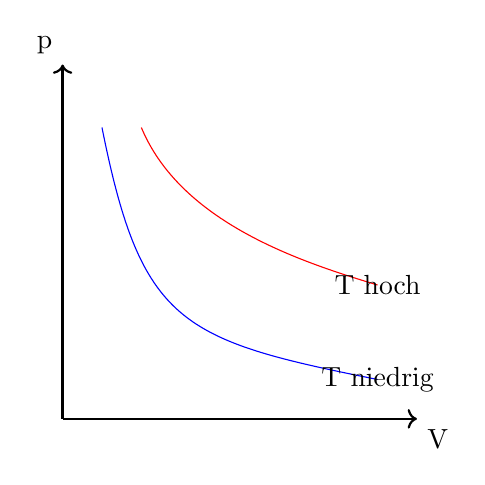
\begin{tikzpicture}
    \draw[thick,->] (0,0) -- (4.5,0) node[anchor=north west] {V};
    \draw[thick,->] (0,0) -- (0,4.5) node[anchor=south east] {p};
    \draw[blue] (0.5 ,3.7) .. controls (1 ,1.2) and (1.5 ,1) .. (4 ,0.5) node[] {\textcolor{black}{T niedrig}};
    \draw[red] (1 ,3.7) .. controls (1.5 ,2.5) and (3 ,2) .. (4 ,1.7) node[] {\textcolor{black}{T hoch}};
\end{tikzpicture}\\
\begin{equation*}
    p \varpropto \frac{1}{V}
\end{equation*}\\
\begin{equation*}
    pV = \mathbf{konst}
\end{equation*}\\
isotherm\\\\
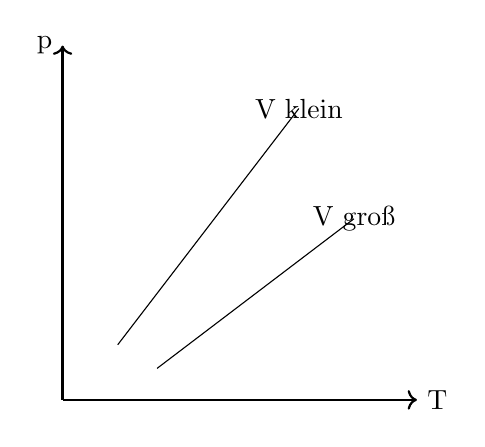
\begin{tikzpicture}
    \draw[thick,->] (0,0) -- (4.5,0) node[anchor=west] {T};
    \draw[thick,->] (0,0) -- (0,4.5) node[anchor=east] {p};
    \draw(0.7 ,0.7) -- (3, 3.7) node[] {V klein};
    \draw(1.2 ,0.4) -- (3.7, 2.3) node[] {V groß};
\end{tikzpicture}\\
\begin{equation*}
    p \varpropto T
\end{equation*}
isochor\newpage
\begin{tikzpicture}
    \draw[thick,->] (0,0) -- (4.5,0) node[anchor=west] {V};
    \draw[thick,->] (0,0) -- (0,4.5) node[anchor=east] {T};
    \draw(0.7 ,0.7) -- (3, 3.7) node[] {p klein};
    \draw(1.2 ,0.4) -- (3.7, 2.3) node[] {p groß};
\end{tikzpicture}\\
\begin{equation*}
    V \varpropto T
\end{equation*}
isobar\\\\
\subsubsection{ideale Gasgleichung $pV = nRT$ bzw. $pV_m = RT$}
$R = 8.314 \frac{\mathrm{J}}{\mathrm{K} \cdot \mathrm{mol}}$ allgemeine Gaskonstante\\
\begin{equation*}
    R = k N_A
\end{equation*}
wobei k die Boltzmannkonstante ist\\\\
$p^o = 1 \mathrm{bar}$\\\\
SATP:
\begin{itemize}
    \item $T=298.15$ K
    \item $p = p^o$
    \item $V_m = 24.789 \frac{\mathrm{dm^3}}{ mol}$
\end{itemize}
STP:
\begin{itemize}
    \item $T=273.15$ K = $0$ °C
    \item $p = p^o$
    \item $V_m = 22.414 \frac{\mathrm{dm^3}}{ mol}$
\end{itemize}
\begin{equation*}
    V(T,p,n) => dV=\left(\frac{\partial V}{\partial T}\right)dT+\left(\frac{\partial V}{\partial p}\right)dp+\left(\frac{\partial V}{\partial n}\right)dn
\end{equation*}
die partiellen Ableitungen sind:\\
thermische Ausdehnung, Komprassibilität, molares Volumen\\
\subsection{kinetische Gastheorie}
\begin{tikzpicture}
    \pgfmathsetmacro{\cubex}{7}
    \pgfmathsetmacro{\cubey}{4}
    \pgfmathsetmacro{\cubez}{4}
    \draw (0,0,0) -- ++(-\cubex,0,0) -- ++(0,-\cubey,0) -- ++(\cubex,0,0) -- cycle;
    \draw (0,0,0) -- ++(0,0,-\cubez) -- ++(0,-\cubey,0) -- ++(0,0,\cubez) -- cycle;
    \draw (0,0,0) -- ++(-\cubex,0,0) -- ++(0,0,-\cubez) -- ++(\cubex,0,0) -- cycle;
\end{tikzpicture}\\
in diesem Raum bewegen sich kleine Gasteilchen.
\begin{itemize}
    \item Mittlere Geschwindigkeit $<v>$
    \item Stöße elastisch
\end{itemize}
Parameter:
\begin{itemize}
    \item Fläche $A$
    \item Volumen $V$
    \item Teilchenanzahl $N$
\end{itemize}
Zahl der Stöße in einer kleinen Zeit $dt$:
\begin{equation*}
    \frac{1}{6} \frac{N}{V}A\langle v\rangle dt
\end{equation*}
Impulsübertragung:
\begin{equation*}
    2m\langle v \rangle
\end{equation*}
Übertragender Impuls:
\begin{equation*}
    dp_A = \frac{1}{3}\frac{N}{V}Am \langle v \rangle ^2 dt
\end{equation*}
Wichtig: $p_A$ ist hier der Impuls
\begin{equation*}
    \frac{dp_A}{dt}=\frac{d\left(mv\right)}{dt}=m\frac{dv}{dt}=ma=F
\end{equation*}
\begin{equation*}
    p = \frac{F}{A}=\frac{1}{3}\frac{N}{V}m\langle v\rangle ^2= \frac{1}{3}\frac{N}{V}m \langle v^2 \rangle
\end{equation*}
Wichtig: $p$ ist hier wieder der Druck
\begin{equation*}
    p=\frac{1}{3}\frac{N}{V}m\left\langle v^2 \right\rangle 
\end{equation*}
\\
Für 1 Mol:
\begin{equation*}
    pV_m=\frac{1}{3}N_Am\langle v^2\rangle = \frac{2}{3}N_AE_{kin}=RT
\end{equation*}
\begin{equation*}
    \sqrt{\langle v^2 \rangle} = \sqrt{\frac{3RT}{M}}
\end{equation*}
\\
Stoßzahl:
\begin{equation*}
    z_1=\sqrt{2}\langle v\rangle \sigma \frac{N}{V}
\end{equation*}
Wobei $\sigma$ die Kriesfläche eines Zylinders ist, in welchem sich das Tielchen fortbewegt.\\
Mittlere freie Wellenlänge: 
\begin{equation*}
    \lambda = \frac{\langle v \rangle}{z_1}=\frac{1}{\sqrt{2}\sigma\frac{N}{V}}
\end{equation*}
\begin{equation*}
    pV = nRT; R = N_Ak_B; n=\frac{N}{N_A}
\end{equation*}
damit:
\begin{equation*}
    \frac{N}{V}=\frac{p}{k_BT}=\frac{1}{\sqrt{2}\sigma\frac{p}{k_BT}}
\end{equation*}
\subsection{Intermolekulare Wechselwirkungen}
elektrischer Dipol.\\
\begin{center}
    \chemfig{H-Cl}
\end{center}
Bei \ce{H} liegt $\delta^+$, bei \ce{Cl} $\delta^-$ somit geht $\vec{\mu}$ von \ce{Cl} zu \ce{H}, von $\delta^-$ zu $\delta^+$\\
\begin{equation*}
    \vec{\mu} = q \vec{R}
\end{equation*}
Wobei $q$ die Ladung ist und $\vec{R}$ der Abstand\\\\
induzierter Dipol:
\begin{equation*}
    \vec{\mu_{ind}}=\alpha \vec{E}
\end{equation*}
Wobei $\alpha$ die Polarisierbarkeit ist und $\vec{E}$ das elektrische Feld.\\
\begin{center}
    $\cdot$\chemfig{H-H}$\cdot$ \ce{->} $\cdot$$\cdot$\chemfig{H-H}
\end{center}
Momentanes Dipolmoment.\\\\
Es gibt folgende Wechselwirkungen:
\begin{itemize}
    \item elektirscher Dipol - elektrischer Dipol
    \item elektrischer Dipol - induzierter Dipol
    \item momentaner Dipol - induzierter Dipol
\end{itemize}
Alle Dipol-Dipol-Wechselwirkungen \textcolor{gray}{(Van-der-Waals-Wechselwirkungen)}\\
$E_{WW} \propto 1\frac{1}{R^6}$\\
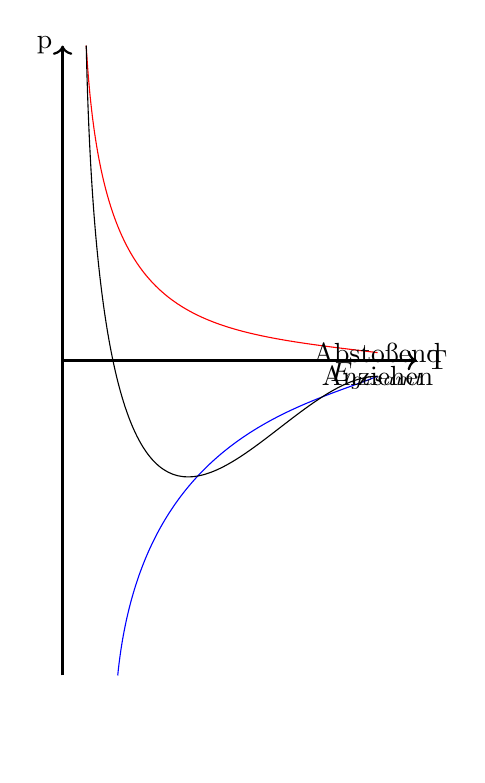
\begin{tikzpicture}
    \draw[thick,->] (0,4) -- (4.5,4) node[anchor=west] {T};
    \draw[thick,->] (0,0) -- (0,8) node[anchor=east] {p};
    \draw[red] (0.3 ,8) .. controls (0.5 ,4.5) and (1.5 ,4.4) .. (4 ,4.1) node[] {\textcolor{black}{Abstoßend}};
    \draw[blue] (0.7 ,0) .. controls (1 ,3) and (3 ,3.4) .. (4 ,3.8) node[] {\textcolor{black}{Anziehen}};
    \draw (0.3 ,8) .. controls (0.5 ,-1) and (2.5 ,3.8) .. (4 ,3.8) node[] {\textcolor{black}{$E_{gesamt}$}};
\end{tikzpicture}
\begin{equation*}
    E_{gesamt}=4\epsilon\left\{\left(\frac{r_0}{R}\right)^{12}-\left(\frac{r_0}{R}\right)^6\right\}
\end{equation*}
Lennard-Jones-Potential, wobei $\epsilon$ mol. Parameter: $\mu, \alpha$\\
Definitiv eine wichtige Gleichung.
\subsection{Reale Gase}
Kompressabilitätsfaktor:
\begin{equation*}
    Z=\frac{pV}{nRT}=1+\dots
\end{equation*}\\
Lösugsansätze:
\begin{itemize}
    \item Korrekturterme $\rightarrow$ Van der Waals Gasgleichung
    \item Reihenenwicklung $\rightarrow$ Virial Gleichung
\end{itemize}
\subsubsection{Van der Waals Gleichung}
\begin{itemize}
    \item[1)] Eigenvolumen\\ Kovolumen: $\frac{\frac{4}{3}\pi\left(2r\right)^3}{2}=4V_{Molek.} \Rightarrow p=\frac{nRT}{V-nb}$ wobei $b=4V_{Molek.}N_A$
    \item[2)] Anziehung der Moleküle: $-a\left(\frac{n}{V}\right)^2 \Rightarrow p=\frac{nRT}{V-nb}-a\left(\frac{n}{V}\right)^2$\\$p=\frac{RT}{V_m-b}-\frac{a}{V_m^2}$
\end{itemize}
\subsubsection{Virialgleichung:}
\begin{equation*}
    Z = 1 + B_p(T)\cdot p + C_p(T)p^2 + \dots
\end{equation*}
Wobei $B_p(T)$ der zweite Virialkoeffizient folgendes beinhaltet bzw. davon abhängig ist:
\begin{itemize}
    \item Eigenvolumen
    \item Intermolekulare Wechselwirkungen
    \item Temperatur
\end{itemize}
\vspace*{1cm}
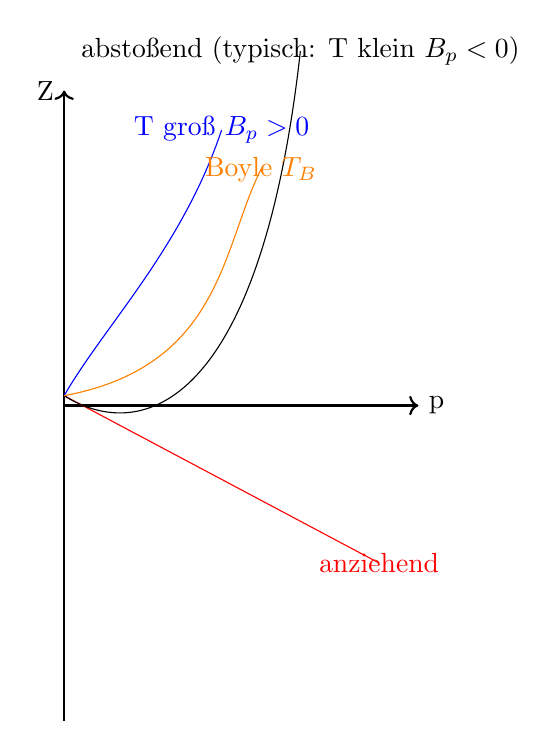
\begin{tikzpicture}
    \draw[thick,->] (0,4) -- (4.5,4) node[anchor=west] {p};
    \draw[thick,->] (0,0) -- (0,8) node[anchor=east] {Z};
    \draw[red] (0,4.125) -- (4, 2) node[] {anziehend};
    \draw (0 ,4.125) .. controls (1 ,3.5) and (2.5 ,4) .. (3 ,8.5) node[] {abstoßend (typisch: T klein $B_p < 0$)};
    \draw[blue] (0 ,4.125) .. controls (0.5 ,5) and (1.5 ,6) .. (2 ,7.5) node[] {T groß $B_p > 0$};
    \draw[orange] (0 ,4.125) .. controls (2 ,4.5) and (2 ,6) .. (2.5 ,7) node[] {Boyle $T_B$};
\end{tikzpicture}
\begin{equation*}
    Z = 1 + \frac{B_V(T)}{V} + \frac{C_V(T)}{V_m^2} + \dots
\end{equation*}
\subsubsection{Kondensation}
p,V-Diagramm\\
\subsubsection{Kritischer Punkt}
\begin{equation*}
    V_{m,g} = V_{m,l}
\end{equation*}
\begin{equation*}
    p_g = p_l
\end{equation*}
$T > T_{Krit}$ nur Gas\\
da $p \approx p_l$ überkritischen Fluid\\
\ce{CO2} $T_{Krit}=31 \, \mathrm{^\circ C}$\\\\
Kritische Größen:
\begin{itemize}
    \item $T_{Krit}$
    \item $p_{Krit}$
    \item $V_{Krit}$
\end{itemize}
\vspace*{1cm}
\begin{equation*}
    V_{red} = \frac{V_m}{V_{m,Krit}} \mathrm{(reduziertes Volumen)}
\end{equation*}
\begin{equation*}
    p_{red} = \frac{p}{p_{Krit}} \mathrm{(reduzierter Druck)}
\end{equation*}
\begin{equation*}
    T_{red} = \frac{T}{T_{Krit}} \mathrm{(reduzierte Temperatur)}
\end{equation*}

\section{Erster Hauptsatz der Thermodynamik}
\subsection{Arbeit, Wärme und Energie}
Energie $E$: Fähigkeit Arbeit zu verrichten $E [\mathrm{J}]$\\
\begin{itemize}
    \item[$\hookrightarrow$] Energieänderung $\Delta E$:
    \begin{itemize}
        \item Leistung von Arbeit $w [\mathrm{J}]$
        \item Austausch von Wärme $q [\mathrm{J}]$
    \end{itemize}
\end{itemize}
Vorzeichen ($q$, $w$) positiv, wenn dem System Energie zugefügt wird.\\
\subsubsection{Arbeit = Kraft $\cdot$ Weg}
\begin{equation*}
    w = \vec{F} \cdot \vec{s} = \left\lvert \vec{F} \right\rvert \left\lvert \vec{s} \right\rvert \cos \varphi
\end{equation*}
$\hookrightarrow "\cdot"$ ist hier ein Skalarprodukt.\\
$\hookrightarrow "\varphi"$ ist hier der Winkel zwischen Kraft und Weg.\\\\
Allgemein:
\begin{equation*}
    F \neq \mathrm{konstant}; dw = \vec{F} \cdot d\vec{s}
\end{equation*}
Integration:
\begin{equation*}
    w = \int_{A}^{E}  \,dw = \int_{s_1}^{s_2}  \vec{F}\cdot d\vec{s}\,dw
\end{equation*}
\subsubsection{Volumenarbeit}
Volumenarbeit wird immer wie folgt geleistet:
\begin{itemize}
    \item am System
    \item gegen einen äußeren Druck
\end{itemize}
\begin{equation*}
    dw = \vec{F} \cdot d\vec{z}
\end{equation*}
Es gilt $p_{ex} = \frac{F}{A}$ und $dz = \frac{dV}{A}$, somit:
\begin{equation*}
    dw = p_{ex}A \frac{dV}{A}
\end{equation*}
\begin{equation*}
    dw = -p_{ex} dV
\end{equation*}
Kraft und Weg entgegengesetzt.
\begin{equation*}
    W = - \int_{z_1}^{z_2} F\,dz = - \int_{V_A}^{V_E} p_{ex} \,dV 
\end{equation*}
\textbf{Beispiel 1} (Ein Ballon)
\begin{equation*}
    p_{ex} = 0, w = ? \rightarrow w = - \int_{V_A}^{V_E} p_{ex} \, dV = 0; \text{ Freie Expansion}
\end{equation*}
\textbf{Beispiel 2}
\begin{equation*}
    p_{ex} = \text{konst.}, w = -\int_{V_A}^{V_E} p_{ex} \, dV = - p_{ex} \int_{V_A}^{V_E} \, dV = -p_{ex}(V_E-V_A) = -p_{ex}\Delta V
\end{equation*}
\textbf{Beispiel 3} isotherme, reversible Expansion
\begin{equation*}
    T = \text{konst},\,p_{ex}=p_{in},\,T_{ex} = T_{in}
\end{equation*}
\begin{equation*}
    w = -\int_{V_A}^{V_E}p\,dV = -nRT \int_{V_A}^{V_E} \frac{1}{V} \,dV = nRT \ln(V) \vert_{V_A}^{V_E} = -nRT(\ln(V_E)-\ln(V_A)) = -nRT\ln\left(\frac{V_E}{V_A}\right)
\end{equation*}
\begin{equation*}
    |w_{rev}|_{p_{in} = p_{ex}} > |w_{innen}|_{p_{ex}=\text{konst.}}
\end{equation*}
\subsubsection{Wärme}
\begin{equation*}
    T_{System} = T_S,\,T_{Umgebung} = T_U
\end{equation*}
\begin{equation*}
    T_S > T_U
\end{equation*}
Somit muss eine Wärmemenge $q$ ausgetauscht werden.\\
Wenn keine Phasenänderungen und keine chemische Reaktionen stattfinden:
\begin{equation*}
    q \varpropto C \Delta T
\end{equation*}
Wobei $C$ die Wärmekapazität ist.\\
Um nun die intensiven Zustandsgröße Wärmekapazität zu einer extensiven Zustandsgröße zu machen, wird die spezifische Wärmekapazität berechnet:
\begin{equation*}
    C_S = \frac{C}{m}
\end{equation*}
Oder die molare Wärmekapazität:
\begin{equation*}
    C_m = \frac{C}{n}
\end{equation*}

\subsection[innere Energie 1.HS]{innere Energie und der 1. Hauptsatz}
Gesamtenergie = äußere Energie $\leftrightarrow$ äußere Koordinaten (Höhe) + Innere Energie $\leftrightarrow$ innere Koordinaten ($p,V,T,n$)\\
Änderung der inneren Energie (Zustandsgröße, extensive Größe)
\begin{equation*}
    \Delta U = U_E - U_A = q + w
\end{equation*}
1. Hauptsatz (ab)geschlossene Systeme\\
\begin{equation*}
    U_1 (\text{Zustand 1}) \ce{<=>[{Weg 1}][{Weg 2}]} U_2 (\text{Zustand 2}) 
\end{equation*}
$U$ muss eine Zustandsgröße sein, sonst wäre ein perpetum mobile möglich.\\
adiabatische Prozesse
\begin{equation*}
    q = 0 \rightarrow \Delta U = w
\end{equation*}
isochor:
\begin{equation*}
    \Delta V = 0 \rightarrow p\Delta V = 0, \, w = 0 \rightarrow \Delta U = q
\end{equation*}
abgeschlossen
\begin{equation*}
    \Delta U = 0
\end{equation*}
Zustandsgröße $U$\\
Weggröße $q,\,w$\\
Änderung:
\begin{equation*}
    dU = \delta q + \delta w
\end{equation*}
Endliche Änderung:
\begin{equation*}
    \Delta U = U_E - U_A = \int_{U_A}^{U_E} \,dU
\end{equation*}
\begin{equation*}
    q=\int_{A}^{E} \delta q \neq q_e - q_a = \Delta q
\end{equation*}
$K,\,n,\,p,\,V\,T$ (S)
\subsubsection{thermische zustandsgleichungen \textcolor{gray}{($pV=nRT$)}}
kalorische zustandsgleichung:
\begin{equation*}
    U = f(V,\,T) ?
\end{equation*}
totales Differential:
\begin{equation*}
    dU = \left(\frac{\partial U}{\partial T}\right)_V\,dT+\left(\frac{\partial U}{\partial V}\right)_T\,dV
\end{equation*}
Verknüpfung mit dem 1. Hauptsatz $dU = \delta q + \delta w$\\
Wenn nur Volumenarbeit:
\begin{equation*}
    -p_{ex}\,dV + \delta q = \left(\frac{\partial U}{\partial T}\right)_V\,dT+\left(\frac{\partial U}{\partial V}\right)_T\,dV
\end{equation*}
Bei isochoren Prozessen: $dV = 0$
\begin{equation*}
    \delta q = \left(\frac{\partial U}{\partial T}\right)_V \,dT = C_V \,dT \Rightarrow dU = C_V \,dT
\end{equation*}
Da $\left(\frac{\partial U}{\partial T}\right)_V = C_V$ ist, \textcolor{gray}{($C_V =$ Wärmekapazität bei konstantem Volumen)}\\
Für einatomige Gase:
\begin{equation*}
    U_m = N_A\langle E_{kin}\rangle = \frac{3}{2}RT \rightarrow C_V,m = \left(\frac{\partial U_m}{T}\right)_V = \frac{3}{2}R = 24,9 \mathrm{\frac{J}{K \cdot mol}}
\end{equation*}

\subsubsection{Freie Expansion}
empirisch $q = 0$\\
$p_{ex}=0 \rightarrow w=0$\\
$\hookrightarrow \Delta U =0$\\
somit
\begin{equation*}
    dU = \left(\frac{\partial U}{\partial T}\right)_V\,dT+\left(\frac{\partial U}{\partial V}\right)_T\,dV = 0
\end{equation*}
Wobei $\left(\frac{\partial U}{\partial V}\right)_T\,dV$ der Binnendruck $\pi_T$ ist.\\
Wenn isotherm:
\begin{equation*}
    dT = 0 \rightarrow \left(\frac{\partial U}{\partial V}\right)_V = 0
\end{equation*}
$\hookrightarrow$ ideales Gas
\begin{equation*}
    dU = D_V\, dT + 0
\end{equation*}
Ideales Gas.\\
\begin{equation*}
    dU = C_V\, dT + \pi_T \,dV
\end{equation*}
Reale Gase.\\
\subsection{Enthalpie}
isobare Prozesse:
\begin{itemize}
    \item $dU = \delta q + \delta w$
    \item $(dU)_p = \delta q_p - p d V$
    \item Integration $ \Rightarrow \Delta U = U_E - U_A = q_p - p (V_E - V_A)$
    \item Umschreiben $q_p = ( U_E + pV_E ) - ( U_A + pV_A) = \Delta (U+pV)$
    \item Definition $H = U + pV$ Enthalpie
    \item $dH = dU + d(pV) = dU + pdV + Vdp$\\$= \delta q + \delta w + pdV + Vdp = \delta q - pdV + pdV + Vdp$\\$\Rightarrow dH = \delta q + Vdp$
    \item $H = H(p,T)$
    \item $dH = \left(\frac{\partial H}{\partial T}\right)_p dT + \left(\frac{\partial H}{\partial p} dp\right)$
\end{itemize}

\subsubsection{Temperaturabhängigkeit \textcolor{gray}{(p = konstant)}}
\begin{equation*}
    dH = \delta q_p = \left(\frac{\partial H}{\partial T}\right)_p dT
\end{equation*}
Wobei $\left(\frac{\partial H}{\partial T}\right)_p$ die $C_p$ Wärmekapazität bei konstantem Druck ist\,ideale Gase $C_p - C_V = nR$\\
Für Flüssigkeiten: $\Delta V \approx 0$\\
Für Feststoffe: $\Delta p \approx 0$\\
$\hookrightarrow \Delta H \approx \Delta U,\, C_p = C_V$

\subsubsection{Druckabgängigkeit der Enthalpie \textcolor{gray}{(Entspannung durch Drossel)}}
\begin{itemize}
    \item[] Kompression links $V_A \rightarrow 0$
    \item[] $w = -p\Delta V=-p_a(0-V_A)=pV_A$
    \item[] Espansion rechts
    \item[] $w = -p\Delta V = -p_E(V_E - 0) = -p_EV_E$
    \item[] Gesamtarbeit: $w = p_AV_A-p_EV_E$
    \item[] $\Delta U=U_E-U_E=w=p_aV_A - P_eV_E$
\end{itemize}
Somit
\begin{equation*}
    U_E + p_Ev_E = U_A + p_AV_a
\end{equation*}
\begin{equation*}
    H_E = H_A
\end{equation*}
Dies nennt man einen isenthalpischen Prozess, da die Anfangs- und Endenthalpie gleich sind.\\
totales Differential:
\begin{equation*}
    dH = \left(\frac{\partial H}{\partial T}\right)_p dT = \left(\frac{\partial H}{\partial p}\right)_T dp
\end{equation*}
Hier:
\begin{equation*}
    0 = C_p dT + \left(\frac{\partial H}{\partial p}\right)_T dp
\end{equation*}
Umschreiben:
\begin{equation*}
    \mu = \left(\frac{\partial T}{\partial p}\right)_H = - \frac{1}{C_p}\left(\frac{\partial H}{\partial p}\right)_T
\end{equation*}
Wobei $\mu$ der Joule-Thomson-Koeffizient ist.\\
Kalometrische Zustandsgleichung für $H$:
\begin{equation*}
    dH = C_p dT - \mu C_p dp
\end{equation*}
Wobei $\mu C_p = 0$ für ein ideales Gas ist.

\subsection{Kalorimetrie: Messung von Wärmeeffekten \textcolor{gray}{Schmelzenthalpien und Reaktionsenthalpien}}
Grundlagen:\\
\begin{center}
    \begin{tabular}{c c}
        \hline
        isochor & $q_V = du$\\
        isobar & $q_p = dH$\\
        \hline
    \end{tabular}\\
\end{center}
Kalorimetrie: Bestimmung von $q$ aus $T$-Änderung.\\
\begin{equation*}
    q = C\Delta T
\end{equation*}
$\hookrightarrow$ Wärmekapazität des Kalorimeters, Kalorimeterkonstante\\

\subsubsection{Adiabatisches Bombenkalorimeter}
\begin{itemize}
    \item Kalibrierung
    \item Bekannte Wärmemenge $q = VIt$
    \item Messen Temperaturänderung
\end{itemize}

\subsection{Adiabatisches Verbrennungskalorimeter}
\begin{equation*}
    q_p = C_p \Delta T
\end{equation*}
\begin{equation*}
    q_p + q_{p,ex} = (C_p + C_{p,ex}) \Delta T
\end{equation*}
\begin{equation*}
    C_{p,ex} = \frac{q_{p,ex}}{\Delta T} = \frac{p_{ex}}{\alpha} \rightarrow \Delta H = \int_{T_1}^{T_2} C_{p,ex} \, dT
\end{equation*}
Heizrate:
\begin{equation*}
    \frac{\Delta T}{\Delta t}
\end{equation*}
Heizleistung:
\begin{equation*}
    \frac{q_{p,ex}}{\Delta t} = p_{ex}
\end{equation*}

\subsection{Thermochemie - Wärmeeffekte chemischer Reaktionen}
\begin{equation*}
    q_p = \Delta H,\, \text{chemische Reaktion: } \Delta_R H
\end{equation*}
\begin{equation*}
    \ce{aA + bB -> cC + dD}
\end{equation*}
\begin{equation*}
    \Delta_R H = cH_c + dH_d - (aH_a + bH_b)
\end{equation*}
Es gilt:
\begin{itemize}
    \item[] $\Delta_R H < 0 :$ exotherm
    \item[] $\Delta_R H > 0 :$ endotherm 
\end{itemize}

\subsubsection{Standardreaktionsenthalpie}
\begin{equation*}
    \Delta_RH^0 = \sum\text{ (Produkte) }\nu_i H_{m,i}^0 - \sum\text{ (Edukte) } \nu_i H_{m,i}^0
\end{equation*}
$H_m^0$ Standardenthalpie\\
Standardbildungsenthalpie $\Delta_BH^0$\\
Bildungsenthalpie (Reaktionsenthalpie für die Bildung aus Elementen im Standardzustand) \textcolor{gray}{(Standardzustand heißt: stabilste Form bei $p=1$ bar)}\\
Bei 298 $^\circ$C \ce{Ns_{(g)}, Hg_{(l)}, C} (Graphit)

\subsubsection{Datz von Hess}
\begin{equation*}
    \ce{C_{(s)} + 1/2 O2_{(g)} -> CO_{(g)}} \Delta_R H_1
\end{equation*}
\begin{equation*}
    \ce{CO_{(g)} + 1/2 O2_{(g)} -> CO2_{(g)}} \Delta_R H_2 = -283 \mathrm{\frac{kJ}{mol}}
\end{equation*}
\begin{equation*}
    \ce{C_{(s)} + O2_{(g)} -> CO2_{(g)}} \Delta_R H_3 = -394 \mathrm{\frac{kJ}{mol}}
\end{equation*}
\begin{equation*}
    \Delta_RH_1 + \Delta_RH_2 = \Delta_RH_3 \Leftrightarrow \Delta_RH1 = \Delta_RH_3 - \Delta_RH_2 = -111 \mathrm{\frac{kJ}{mol}}
\end{equation*}

\subsubsection{Kirchhoffsches Gesetz}
\begin{equation*}
    H(T_2) = H(T_1) + \int_{T_1}^{T_2} C_p \, dT = H(T_1)+C_p \Delta T
\end{equation*}
Weg I:
\begin{equation*}
    \Delta H^0 (I) = \Delta_RH^0 (T_1) + \Delta_{Erw} H^0 (T_1 \rightarrow T_2) = \Delta_RH^0(T_1) + (C_{p,m}^0(C) + C_{p,m}(D)) \Delta T
\end{equation*}
Weg II:
\begin{equation*}
    \Delta H^0 (II) = \Delta_{Erw} H^0 (T_1 \rightarrow T_2) + \Delta_RH^0 (T_2) = (C_{p,m}^0 (A) + C_{p,m}^0 (B))\Delta T + \Delta_RH^0 (T_2)
\end{equation*}
\begin{equation*}
    \Delta_RH^0 (T_2) = \Delta_RH^0 (T_1) + (C_{p,m}^0 (C)+C_{p,m}^0 (D)-C_{p,m}^0(A)-C_{p,m}^0(B)) \Delta T = \Delta_RH^0 (T_1) + \Delta_RC_p^0 \Delta T
\end{equation*}

\section{Der 2. Hauptsatz}
\textbf{2. Hauptsatz nach Clausius: Wärme verbreitet nicht spontan von kalt nach warm.}\\
\textbf{2. Hauptsatz nach Kelvin: Kreisprozess, wobei $q$ vollständig in Arbeit $w$ umgesetzt wird ist unmöglich!}

\subsection{Carnotscher Kreisprozess}
\subsubsection{isotherme Prozesse (reversibel) ideales Gas}
\begin{equation*}
    dU = \delta q - pdV = \left(\frac{\partial U}{\partial T}\right)_V \, dT + \left(\frac{\partial U}{\partial V}\right)_T \, dV
\end{equation*}
$\Rightarrow dU = 0$ und $\delta q = pdV$\\
\begin{itemize}
    \item[] Expansion: $dV>0$
    \item[] Kompression: $dV<0$
\end{itemize}
Für den Prozess $V_A \rightarrow V_E$ gilt:
\begin{equation*}
    W = - \int_{V_A}^{V_E} p \, dV = -nRT \int_{V_A}^{V_E} \frac{1}{V} \, dV = -nRT \ln\left(\frac{V_E}{V_A}\right) = -q_{Exp}
\end{equation*}
Für den Prozess $V_E \rightarrow V_A$ gilt:
\begin{equation*}
    W = -nRT \ln\left(\frac{V_A}{V_E}\right)=-q_{Kom}
\end{equation*}

\subsubsection{Adiabatische Prozesse (reversibel) \textcolor{gray}{($q=0$)}}
\begin{itemize}
    \item[] Bei Expansion $W < 0 \Rightarrow \Delta U < 0$
\end{itemize}
\begin{equation*}
    \Delta U = \int_{T_1}^{T_2} C_V dT = C_V \Delta T
\end{equation*}
\begin{equation*}
    \Delta U_{\mathrm{adiabatisch}} = C_V \Delta T
\end{equation*}
\begin{equation*}
    \Delta U = q + w \Rightarrow w = C_V \Delta T
\end{equation*}

\subsubsection{Adiabatengleichung}
\begin{equation*}
    dU = D_V \,dT = -p\,dV = - \frac{nRT}{V} \, dV
\end{equation*}
Um dies nun zu integrieren, ist eine Trennung der Variablen notwendig.
\begin{equation*}
    -nR \frac{dV}{V} = C_V \frac{dT}{T}
\end{equation*}
\begin{equation*}
    -R \int_{V_A}^{V_E} \frac{1}{V}\,dV = \int_{T_A}^{T_E} \frac{1}{T} \, dT
\end{equation*}
Mit der Annahme $C_V \neq C_V (T)$ ist folgendes Möglich:
\begin{equation*}
    -nR \ln\left(\frac{V_E}{V_A}\right) = C_V \ln\left(\frac{T_E}{T_A}\right)
\end{equation*}
Einsetzen von $nR = C_p - C_V$:
\begin{equation*}
    - \frac{C_p - C_V}{C_V} \ln\left(\frac{V_E}{V_A}\right) = ln\left(\frac{T_E}{T_A}\right), \, \gamma = \frac{C_p}{C_V} > 1
\end{equation*}
\begin{equation*}
    (\gamma - 1)\ln\left(\frac{V_A}{V_E}\right) = \ln\left(\frac{T_E}{T_A}\right)
\end{equation*}
\begin{equation*}
    \ln\left(\frac{V_A}{V_E}\right)^{\gamma-1} = \ln\left(\frac{T_E}{T_A}\right)
\end{equation*}
Dies ist die Adiabatengleichung.\\
Mit $T = \frac{pV}{nR}$ ist noch folgende Umformung möglich:
\begin{equation*}
    p_EV_E^\gamma = p_AV_A^\gamma
\end{equation*}

\subsubsection{Carnotscherkreisprozess}
\begin{center}
    \begin{tabular}{c c c}
        \hline
        Schritt & q & w\\
        \hline
        \\
        1 & $q_w=nRT_w\ln\frac{V_B}{V_A}$ & $w_1 = -nRT\ln\frac{V_B}{V_A} < 0$\\
        \\
        2 & $q_2=0$ & $w_2=C_V\Delta T = C_V(T_K-T_w) < 0$\\
        \\
        3 & $q_k$ = $nRT\ln\frac{V_D}{V_C}$ & $w_3 = -nRT \ln\frac{V_D}{V_C} > 0$\\
        \\
        4 & $q_4 = 0$ & $w_4 = C_V\Delta T = C_V(T_W-T_K) > 0$\\
        \hline
    \end{tabular}
\end{center}
\begin{eqnarray*}
    \Delta U = q+w=q_w+q_k+w_1+w_2+w_3+w_4 = 0 \Rightarrow w=-(q_w+q_k)\\
    w=-nRT_w\ln\frac{V_B}{V_A}+C_V(T_K-T_W)-nRT_k\ln\frac{V_D}{V_C}+C_V(T_W-T_K)\\
    =-nRT_W\ln\frac{V_B}{V_A}-nRT_K\ln\frac{V_D}{V_C}\\
    \frac{T_W}{T_K}=\left(\frac{V_C}{V_B}\right)^{\gamma-1}=\left(\frac{V_D}{V_C}\right)^{\gamma-1} \Rightarrow \left(\frac{V_D}{V_C}\right)=\left(\frac{V_A}{V_B}\right)\,\text{ in überstehende Gleichung:}\\
    w = -nRT_W\ln\frac{V_B}{V_A}-nRT_K\ln\frac{V_A}{V_B}\\
    = -nRT(T_W-T_K)\ln\frac{V_B}{V_A}
\end{eqnarray*}

\subsubsection{Wärmekraftmaschine}
\begin{itemize}
    \item Dampfturbine
\end{itemize}

\subsubsection{Wirkungsgrad}
\begin{eqnarray*}
    \eta = \frac{\text{geleistete Arbeit}}{\text{aufgenommene Wärme}}=\frac{-w}{q_w}=\frac{T_W-T_K}{T_W}=1-\frac{T_K}{T_W} < 1\\
    w=-nRT(T_W-T_K)\ln\frac{V_B}{V_A}\\
    q_w = nRT_W\ln\frac{V_B}{V_A}
\end{eqnarray*}

\section{Entropie}
\begin{eqnarray*}
    q_w=nRT_W\ln\frac{V_B}{V_A} \Leftrightarrow \frac{q_w}{T_w}=nR\ln\frac{V_B}{V_A}\\
    q_k = nRT_K\ln\frac{V_D}{V_C} \Leftrightarrow \frac{q_k}{T_K}=nR\ln\frac{V_D}{V_C}\\
    \frac{q_w}{T_W}+\frac{q_k}{T_K}=nR\ln\frac{V_B}{V_C}+nR\ln\frac{V_D}{V_C}=0\\
    \sum \frac{q_{rev}}{T}=0
\end{eqnarray*}

\subsubsection{Definition der Zustandsgröße Entropie $S$}
\begin{eqnarray*}
    dS_{Sys}=\frac{q_{rev}}{T}\\
    \Delta S_{Sys}=\frac{q_{rev}}{T}
\end{eqnarray*}
Für die Umgebung gilt:
\begin{eqnarray*}
    V = \text{konst.} \Rightarrow w = 0\\
    \Rightarrow dU = \partial q\\
    \\
    dS_{Sys} = \frac{\partial q_{Umg}}{T_{Umg}}
\end{eqnarray*}

\subsubsection{Isotherme ($\Delta T=0$), reversiple Expansion}
\begin{eqnarray*}
    \Delta_{Sys}=\int_{A}^{E}\frac{\partial q_{res}}{T} = \frac{1}{T} \int_{A}^{E} \partial q_{res} = \frac{q_{res}}{T}\\
    q = nRT\ln\frac{V_E}{V_A}\\
    \Rightarrow \Delta_{Sys} = nR\ln\frac{V_E}{V_A}>0
\end{eqnarray*}

\subsubsection{adiabatische, reversible Expansion}
\begin{equation*}
    \Delta_{Sys} = 0,\,q_{res}=0
\end{equation*}

\subsubsection{Isobarer Phasenübergang}
\begin{eqnarray*}
    \Delta p = 0 \Rightarrow \partial q_p = dH\\
    \Delta S_{Sys} = \frac{q_p}{T_{Trans}}=\frac{\Delta_{Trans} H}{T_{Trans}}
\end{eqnarray*}

\subsubsection{Isobare Erhitzung}
\begin{eqnarray*}
    \Delta p = 0,\,\partial q = dH = C_p\,dT\\
    \Delta S_{Sys} = \int_{A}^{E}  \frac{\partial q_{rev}}{T} = \int_{T_A}^{T_E} C_p \frac{1}{T}\,dT = C_p\ln\frac{T_E}{T_A}
\end{eqnarray*}

\subsubsection{Beliebiger Kreisprozess ist die Summe von Carnotprozessen}
\begin{eqnarray*}
    \oint \frac{\partial q_{rev}}{T}=0\\
\end{eqnarray*}

\subsubsection{Wärme Austausch zwischen einem warmen und einem kalten Reservoir}
\begin{center}
    \begin{tabular}{l c c c}
        \hline
        \rule{0pt}{15pt}&Wärme A&WärmeB&Arbeit\\
        \hline
        \rule{0pt}{15pt}hin(irreversibel)&$-q_k$&$q_k$&0\\
        \rule{0pt}{15pt}zurück(reversibel)&$q_w$&$-q-k$&$-nR(T_W-T_K)\ln\frac{V_B}{V_A} > 0$\\
        \hline
        \rule{0pt}{15pt}Summe&$q_w-Q_k>0$&0&$-nR(T_W-T_K)\ln\frac{V_B}{V_A} < 0$\\
        \rule{0pt}{15pt}&plus an Wärme&&Minus an Arbeit\\
        \hline
    \end{tabular}
\end{center}

\begin{center}
    \begin{tabular}{l c c c}
        \hline
        \rule{0pt}{15pt}&$\Delta U_{Sys}$&Wärme umgebung & Arbeit Umgebung\\
        \hline
        \rule{0pt}{15pt}hin(irrev)&$0=-q_1+p_z\Delta V$&$-q_1 = -p_z\Delta V$& $-p_E\Delta v$\\
        \rule{0pt}{15pt}rück(rev)&$0=-q_2+nRT\ln\frac{V_E}{V_A}$&$q_w0nRT\ln\frac{V_E}{V_A}$&$-nRT\ln\frac{V_E}{V_A}$\\
        \hline
        \rule{0pt}{15pt}Summe&0&$nRT\ln\frac{V_E}{V_A}-p_{ex}\Delta V > 0$&$-nRT\ln\frac{V_E}{V_A}-p_E\Delta V < 0$
    \end{tabular}
\end{center}

\begin{eqnarray*}
    \Delta S_W=-\frac{|q|}{T_W}\\
    \Delta S_K=\frac{||q|}{T_K}\\
    \Delta S_{Ges}=\Delta S_W + \Delta S_K = q(\frac{1}{T_K}-\frac{1}{T_W}) >0\\
    \Delta S_{Ges} > 0 \text{ bei freiwilligen Prozessen}
\end{eqnarray*}

\subsection{Volumenänderung}
$\rightarrow$ Irreversibel\\
\begin{eqnarray*}
    \Delta S_{Umg} = ?\\
    \Delta S_{Sys} = ?\\\
    \text{Umgebung} q = -w\\
    w = -\int_{V_A}^{V_E}p_{ex}\,dV=-p_{ex}\Delta V\\
    \Delta S_{Umg} = \frac{q_{Umg}}{T_{Umg}} = \frac{-q}{T_{Umg}}=\frac{-p_{ex}\Delta V}{T_{Umg}} < 0\\
    \Delta S_{Sys} = \frac{q_{rev}}{T} = \frac{-w}{T} = \frac{nRT\ln\frac{V_E}{V_A}}{T} = nR\ln\frac{V_E}{V_A} > 0\\\\
    \Delta S_{Ges} = \Delta S_{Sys}+\Delta D_{Umg} > 0
\end{eqnarray*}

\subsubsection{Clausiussche Ungleichung}
\begin{eqnarray*}
    \text{reversibel: } dU = \delta q_{rev} - p\,dV\\
    \text{irreversibel: } dU = \delta q - p_{ex}\,dV\\
    \delta q_{rev} - \delta q = (p-p_{ex})\,dV\\
    \Rightarrow \delta q_{rev} - \delta q \geqslant 0\\
    dS = \frac{\delta q_{rev}}{T} \Leftrightarrow \delta q_{rev} = T\,dS\\
    T\,dS \geqslant \delta q\\
    \text{Clausiussche Ungleichung: } dS_{Sys} \geqslant \frac{\delta q}{T}\\
    \Delta S \geqslant \frac{q}{T}\\
    > \text{ für irreversible Prozesse } = \text{ für reversible}
\end{eqnarray*}

\begin{center}
    \begin{tabular}{l c c}
        \hline
        \rule{0pt}{15pt}&reversibel&irreversibel\\
        \hline
        \rule{0pt}{15pt}geschlossen ($q\neq 0$)&$\Delta S = \frac{q_{rev}}{T}$&$\Delta S-\frac{q_{irrev}}{T} > 0$\\
        \rule{0pt}{15pt}abgeschlossen ($q=0$)&$\Delta S = 0$& $\Delta S > 0$\\
    \end{tabular}
\end{center}
Beispiel: Universum\\
reversible Prozesse Entropie des Universums bleibt gleich\\
irreversible (spontante) Prozesse, die Entropie nimmt zu.\\

\section{3.Hauptsatz der Thermodynamik}
Empirisch Nernst'sche Wärmetheorie
\begin{equation*}
    \lim_{T\rightarrow 0} \Delta S = 0
\end{equation*}
Reaktion:
\begin{equation*}
    \Delta S = \sum_{i} \nu_i S_{m,i} \Rightarrow \lim_{T\rightarrow 0} \Delta S = 0,\, S(\mathrm{Edukte}) \approx S(\mathrm{Produkte})
\end{equation*}
\begin{equation*}
    S_m (T=0\,\mathrm{K}) \text{ ist stoffunabhängig}
\end{equation*}
Postulieren $S_m (T=0\,\mathrm{K})=0$ für perfekte Kristalle\\\\
Beispiel:\\
Phasenübergang $\ce{S}(\beta) \rightarrow \ce{S}(\alpha)$\\
\begin{equation*}
    \Delta S = \int^{E}_{A} \frac{\delta q_{rev}}{T}=\int_{300K}^{0K}c_p\frac{1}{T}\,dT
\end{equation*}
\subsection*{Freie Energiegrößen}
Smausius Ungleichung
\begin{equation*}
    dS > \frac{\delta q}{T} \Leftrightarrow TdS-\delta q > 0\,\text{ (spontante Prozesse)}
\end{equation*}
isochor:
\begin{eqnarray*}
    dU = \delta q_V\\
    dU-T\,dS < 0\\
    A = U-TS\,\text{ Freie Energie, Helmholtz-Energie (Zustandsgröße)}\\
    dA = dU-d(TS) = dU - T\,dS-S\,dT\\
\end{eqnarray*}
\begin{itemize}
    \item isotherm $dA = dU-T\,dS$
    \item spontan $dA<0$
    \item nicht spontan $dA > 0$
    \item Gleichgewicht $dA = 0$
\end{itemize}
\begin{eqnarray*}
    T\,dS-\delta q \geq 0\\
    dU = \delta q + \delta w\\
    \Rightarrow \delta w \geq dU - T\,dS\\
    \delta w_{max} = dU-T\,dS = dA (V=T=\mathrm{konst})
\end{eqnarray*}
$A$ ist der maximale für Leistung von Arbeit verfügbarer Teil der inneren Energie.\\
\\isobar:
\begin{eqnarray*}
    dH = \delta q_p\\
    \text{freiwillig: } dH-T\,dS<0\text{ für reversible: } dH-T\,dS=0\\
    G=H-TS \text{ Freie Enthalpie, HGibbs Energie}\\
    dG = dH-T\,dS-S\,dT\\
    \text{isotherm: } dG=dH-T\,dS \Leftrightarrow \Delta G = \Delta H-T\Delta S\\
    \text{freiwillig: } \Delta G < 0 \text{ exergonisch}\\
    \text{nicht freiwillig } \Delta G > 0 \text{ endergonisch}
\end{eqnarray*}
\section{1. + 2. Hauptsatz}
\begin{eqnarray*}
    dU = \delta w + \delta q \Rightarrow dU = T\,dS-p\,dV \text{ Fundamentalgleichung der inneren Energie}\\
    H=U+pV\Rightarrow dH=dU+p\,dV+V\,dp\Rightarrow dH=T\,dS+V\,dp\,(S,p)\\
    A=U-TS\Rightarrow dA=dU=T\,dS-S\,dT\Rightarrow dA=-S\,dT-p\,dV\,(T,V)\\
    G=H-TS\Rightarrow dG=dH-T\,dS-S\,dT\Rightarrow dG=-S\,dT+V\,dp\,(T,p)
\end{eqnarray*}
\begin{eqnarray*}
    dU=\left(\frac{\partial U}{\partial S}\right)_V\,dS+\left(\frac{\partial U}{\partial V}\right)_S\,dV = T\,dS-p\,dV
\end{eqnarray*}
\subsubsection{Satz von Schwartz}
\begin{eqnarray*}
    \frac{\partial}{\partial x}\left(\frac{\partial f}{\partial y}\right)_x = \frac{\partial}{\partial x}\left(\frac{\partial f}{\partial x}\right)_y\\
    U = U(S,V),\, dU=T\,dS-p\,dV\\
    \frac{\partial}{\partial V}\left(\frac{\partial U}{\partial S}\right)_V = \frac{\partial}{\partial S}\left(\frac{\partial U}{\partial V}\right)_S \Rightarrow \left(\frac{\partial T}{\partial V}\right)_S = -\left(\frac{\partial p}{\partial S}\right)_V
\end{eqnarray*}

\subsubsection{Guggenheim}
\begin{equation*}
    +\begin{array}{c c c}
        S U V\\
        H  A\\
        p G T\\
    \end{array}-
\end{equation*}
\begin{eqnarray*}
    dG = V\,dp+D\,dT\\
    S = -\frac{\partial G}{\partial T} = - \frac{\partial A}{\partial T}
\end{eqnarray*}

\subsubsection{$T$- , $p$-Abhängigkeit von $G$}
\begin{eqnarray*}
    \left(\frac{\partial G}{\partial T}\right)_p = -S\\
    \left(\frac{\partial G}{\partial p}\right)_T = V
\end{eqnarray*}

\subsubsection{$T$-Abhängigkeit von $G$}
\begin{eqnarray*}
    \Delta D = G_E - G_A\\
\end{eqnarray*}
G in Feststoffen nimmt nur langsam ab, in Flüssigkeiten etwas schneller und in Gasen sehr rapide.

\subsubsection{Gibbs-Helmholtz Gleichung}
\begin{eqnarray*}
    \Delta G = \Delta H - T \Delta S\\
    G = H-TS \Leftrightarrow S= -\frac{G-H}{T} \text{ Einsetzen } S=-\frac{\partial G}{\partial T}_p\\
    \left(\frac{\partial G}{\partial T}\right)_p = \frac{G-H}{T}\\
    \frac{\partial}{\partial T}\left(\frac{G}{T}\right) = \frac{1}{T}\frac{\partial G}{\partial T} - \frac{G}{T^2}=\frac{1}{T}\left(\left(\frac{\partial G}{\partial T}\right)-\frac{G}{F}\right)\\
    \frac{\partial}{\partial T}\left(\frac{G}{T}\right) = -\frac{H}{T^2}\\
    \frac{\partial}{\partial T}\left(\frac{\Delta G}{T}\right)_p = -\frac{\Delta H}{T^2}
\end{eqnarray*}
$\rightarrow$ Gibbs-Helmholtz Gleichung

\subsubsection{$p$-Abhängigkeiten $V_{gas}>>V_l>V_s$ bei $T =$konst}
\begin{eqnarray*}
    \int_{G_A}^{G_E}dG = \int_{T_A}^{T_E}-S\,dT+\int_{p_A}^{p_E}V\,dp\\
    \Delta G = \int_{p_A}^{p_E}V\,dp\\
    \text{solid, liquid: } \Delta G = V\Delta p\\
    \text{gas: } \Delta G = \int_{p_A}^{p_E}V_m\,dp=RT\int_{p_A}^{p_E}\frac{1}{p}\,dp=RT\ln\frac{p_E}{p_A}
\end{eqnarray*}

\subsubsection{chemisches Potential}
$G$ extensive Größe\\
$G_m = \frac{G}{n}$ hier ist $n$ die Stoffmenge\\
Gemisch:\\
Chemisches Potential $\mu_i = \left(\frac{\partial G}{\partial n_i}\right)_{p,T,n'}$\\
$G(p,T,n_1,n_2,n_s,\dots,n_k) \Rightarrow dG = \left(\frac{\partial G}{\partial p}\right)_{T,n_i}\,dp+ \left(\frac{\partial G}{\partial T}\right)_{p,n}\,dT+\left(\frac{\partial G}{\partial n_1}\right)_{p,T,n'}\,dn_1+\left(\frac{\partial G}{\partial n_2}\right)_{p,T,n'}\,dn_2$\\
\begin{eqnarray*}
    dG = V\,dp - S\,dT + \sum_{i=1}^{k} \mu_i\,dn_i\\
    T,p = \mathrm{const.} \Rightarrow dG = \sum_{i=1}^{k}\mu_i\,dn_i\\
    G=\sum_{i=1}^{k} \mu_in_i\\
    dU=T\,dS-p\,dV\\
    S,V=\mathrm{const.} \Rightarrow dU = \sum_{i=1}^{k} \mu_i\,dn_i \Rightarrow \mu_i = \left(\frac{\partial U}{\partial n_i}\right)_{V,S,n'}
\end{eqnarray*}
\end{document}